\begin{figure}[ht]
\begin{center}
\begin{adjustbox}{width=0.7\textwidth}


\tikzset{every picture/.style={line width=0.75pt}} %set default line width to 0.75pt        

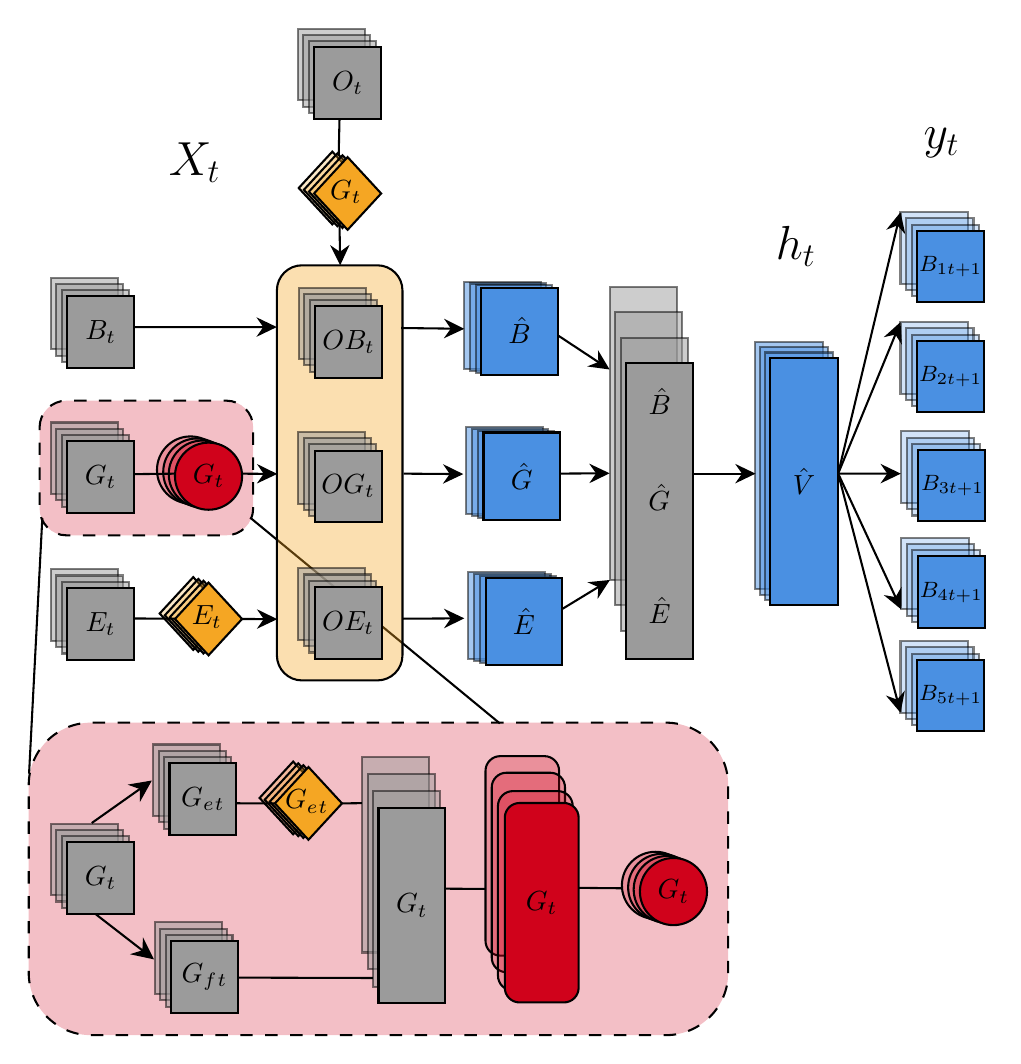
\begin{tikzpicture}[x=0.75pt,y=0.75pt,yscale=-1,xscale=1]
%uncomment if require: \path (0,532); %set diagram left start at 0, and has height of 532

%Shape: Rectangle [id:dp8163589302848298] 
\draw  [color={rgb, 255:red, 0; green, 0; blue, 0 }  ,draw opacity=0.5 ][fill={rgb, 255:red, 74; green, 144; blue, 226 }  ,fill opacity=0.5 ] (471.1,172.6) -- (503.87,172.6) -- (503.87,291.87) -- (471.1,291.87) -- cycle ;
%Shape: Rectangle [id:dp13561622734198409] 
\draw  [color={rgb, 255:red, 0; green, 0; blue, 0 }  ,draw opacity=0.5 ][fill={rgb, 255:red, 74; green, 144; blue, 226 }  ,fill opacity=0.5 ] (473.57,175.18) -- (506.34,175.18) -- (506.34,294.44) -- (473.57,294.44) -- cycle ;
%Shape: Rectangle [id:dp028266783786446537] 
\draw  [color={rgb, 255:red, 0; green, 0; blue, 0 }  ,draw opacity=0.5 ][fill={rgb, 255:red, 74; green, 144; blue, 226 }  ,fill opacity=0.5 ] (476.05,177.76) -- (508.82,177.76) -- (508.82,297.02) -- (476.05,297.02) -- cycle ;
%Shape: Rectangle [id:dp501556684499422] 
\draw  [fill={rgb, 255:red, 74; green, 144; blue, 226 }  ,fill opacity=1 ] (478.52,180.33) -- (511.29,180.33) -- (511.29,299.6) -- (478.52,299.6) -- cycle ;

%Rounded Rect [id:dp7384006244940544] 
\draw  [fill={rgb, 255:red, 208; green, 2; blue, 27 }  ,fill opacity=0.25 ][dash pattern={on 4.5pt off 4.5pt}] (121.33,386.22) .. controls (121.33,369.59) and (134.82,356.1) .. (151.45,356.1) -- (428.22,356.1) .. controls (444.85,356.1) and (458.33,369.59) .. (458.33,386.22) -- (458.33,476.56) .. controls (458.33,493.19) and (444.85,506.68) .. (428.22,506.68) -- (151.45,506.68) .. controls (134.82,506.68) and (121.33,493.19) .. (121.33,476.56) -- cycle ;
%Rounded Rect [id:dp4183866908288403] 
\draw  [color={rgb, 255:red, 0; green, 0; blue, 0 }  ,draw opacity=1 ][fill={rgb, 255:red, 208; green, 2; blue, 27 }  ,fill opacity=0.25 ][line width=0.75]  (341.41,379.33) .. controls (341.41,375.42) and (344.59,372.24) .. (348.5,372.24) -- (369.77,372.24) .. controls (373.68,372.24) and (376.86,375.42) .. (376.86,379.33) -- (376.86,461.25) .. controls (376.86,465.17) and (373.68,468.34) .. (369.77,468.34) -- (348.5,468.34) .. controls (344.59,468.34) and (341.41,465.17) .. (341.41,461.25) -- cycle ;
%Rounded Rect [id:dp3099111807535615] 
\draw  [color={rgb, 255:red, 0; green, 0; blue, 0 }  ,draw opacity=1 ][fill={rgb, 255:red, 208; green, 2; blue, 27 }  ,fill opacity=0.25 ][line width=0.75]  (344.41,387.3) .. controls (344.41,383.4) and (347.58,380.24) .. (351.47,380.24) -- (372.65,380.24) .. controls (376.55,380.24) and (379.71,383.4) .. (379.71,387.3) -- (379.71,469.28) .. controls (379.71,473.18) and (376.55,476.34) .. (372.65,476.34) -- (351.47,476.34) .. controls (347.58,476.34) and (344.41,473.18) .. (344.41,469.28) -- cycle ;
%Rounded Rect [id:dp8381713204360262] 
\draw  [color={rgb, 255:red, 0; green, 0; blue, 0 }  ,draw opacity=1 ][fill={rgb, 255:red, 208; green, 2; blue, 27 }  ,fill opacity=0.25 ][line width=0.75]  (347.41,396.28) .. controls (347.41,392.3) and (350.64,389.08) .. (354.62,389.08) -- (376.23,389.08) .. controls (380.2,389.08) and (383.43,392.3) .. (383.43,396.28) -- (383.43,477.97) .. controls (383.43,481.95) and (380.2,485.18) .. (376.23,485.18) -- (354.62,485.18) .. controls (350.64,485.18) and (347.41,481.95) .. (347.41,477.97) -- cycle ;
%Straight Lines [id:da9948239674954347] 
\draw    (228,257.31) -- (348.33,356.48) ;
%Straight Lines [id:da5479751788470504] 
\draw    (127.88,257.6) -- (121.5,380.65) ;
%Rounded Rect [id:dp3615352313435898] 
\draw  [fill={rgb, 255:red, 208; green, 2; blue, 27 }  ,fill opacity=0.25 ][dash pattern={on 4.5pt off 4.5pt}] (126.56,213.95) .. controls (126.56,206.78) and (132.37,200.97) .. (139.54,200.97) -- (216.49,200.97) .. controls (223.66,200.97) and (229.47,206.78) .. (229.47,213.95) -- (229.47,252.88) .. controls (229.47,260.05) and (223.66,265.86) .. (216.49,265.86) -- (139.54,265.86) .. controls (132.37,265.86) and (126.56,260.05) .. (126.56,252.88) -- cycle ;
%Shape: Circle [id:dp1543780616872943] 
\draw  [fill={rgb, 255:red, 208; green, 2; blue, 27 }  ,fill opacity=0.25 ] (183.13,234.37) .. controls (183.13,225.44) and (190.37,218.2) .. (199.3,218.2) .. controls (208.23,218.2) and (215.47,225.44) .. (215.47,234.37) .. controls (215.47,243.3) and (208.23,250.53) .. (199.3,250.53) .. controls (190.37,250.53) and (183.13,243.3) .. (183.13,234.37) -- cycle ;
%Shape: Circle [id:dp12704022883485055] 
\draw  [fill={rgb, 255:red, 208; green, 2; blue, 27 }  ,fill opacity=0.25 ] (186.13,235.37) .. controls (186.13,226.44) and (193.37,219.2) .. (202.3,219.2) .. controls (211.23,219.2) and (218.47,226.44) .. (218.47,235.37) .. controls (218.47,244.3) and (211.23,251.53) .. (202.3,251.53) .. controls (193.37,251.53) and (186.13,244.3) .. (186.13,235.37) -- cycle ;
%Shape: Circle [id:dp9413162181699031] 
\draw  [fill={rgb, 255:red, 208; green, 2; blue, 27 }  ,fill opacity=0.25 ] (188.8,236.37) .. controls (188.8,227.44) and (196.04,220.2) .. (204.97,220.2) .. controls (213.9,220.2) and (221.13,227.44) .. (221.13,236.37) .. controls (221.13,245.3) and (213.9,252.53) .. (204.97,252.53) .. controls (196.04,252.53) and (188.8,245.3) .. (188.8,236.37) -- cycle ;
%Shape: Circle [id:dp2604605191599928] 
\draw  [fill={rgb, 255:red, 208; green, 2; blue, 27 }  ,fill opacity=1 ] (191.8,237.37) .. controls (191.8,228.44) and (199.04,221.2) .. (207.97,221.2) .. controls (216.9,221.2) and (224.13,228.44) .. (224.13,237.37) .. controls (224.13,246.3) and (216.9,253.53) .. (207.97,253.53) .. controls (199.04,253.53) and (191.8,246.3) .. (191.8,237.37) -- cycle ;

%Rounded Rect [id:dp4954977443195646] 
\draw  [fill={rgb, 255:red, 245; green, 166; blue, 35 }  ,fill opacity=0.36 ] (240.9,147.86) .. controls (240.9,141.18) and (246.32,135.76) .. (253,135.76) -- (289.3,135.76) .. controls (295.98,135.76) and (301.4,141.18) .. (301.4,147.86) -- (301.4,323.66) .. controls (301.4,330.35) and (295.98,335.76) .. (289.3,335.76) -- (253,335.76) .. controls (246.32,335.76) and (240.9,330.35) .. (240.9,323.66) -- cycle ;
%Straight Lines [id:da7142528898407593] 
\draw    (271.06,115.47) -- (271.35,132.76) ;
\draw [shift={(271.4,135.76)}, rotate = 269.03] [fill={rgb, 255:red, 0; green, 0; blue, 0 }  ][line width=0.08]  [draw opacity=0] (9.82,-4.72) -- (0,0) -- (9.82,4.72) -- (6.52,0) -- cycle    ;
%Shape: Rectangle [id:dp4257379299322124] 
\draw  [color={rgb, 255:red, 0; green, 0; blue, 0 }  ,draw opacity=0.5 ][fill={rgb, 255:red, 155; green, 155; blue, 155 }  ,fill opacity=0.5 ] (132.01,282.24) -- (164.26,282.24) -- (164.26,316.76) -- (132.01,316.76) -- cycle ;
%Shape: Rectangle [id:dp21839521574886023] 
\draw  [color={rgb, 255:red, 0; green, 0; blue, 0 }  ,draw opacity=0.5 ][fill={rgb, 255:red, 155; green, 155; blue, 155 }  ,fill opacity=0.5 ] (134.63,285.22) -- (166.88,285.22) -- (166.88,319.74) -- (134.63,319.74) -- cycle ;
%Shape: Rectangle [id:dp4226350391764252] 
\draw  [color={rgb, 255:red, 0; green, 0; blue, 0 }  ,draw opacity=0.5 ][fill={rgb, 255:red, 155; green, 155; blue, 155 }  ,fill opacity=0.5 ] (137.27,288.28) -- (169.53,288.28) -- (169.53,322.79) -- (137.27,322.79) -- cycle ;
%Shape: Rectangle [id:dp06632573802600894] 
\draw  [fill={rgb, 255:red, 155; green, 155; blue, 155 }  ,fill opacity=1 ] (139.86,291.21) -- (172.11,291.21) -- (172.11,325.73) -- (139.86,325.73) -- cycle ;
%Straight Lines [id:da34674908382474934] 
\draw    (271.06,65.57) -- (270.67,83.14) ;
%Shape: Rectangle [id:dp3929589883407535] 
\draw  [color={rgb, 255:red, 0; green, 0; blue, 0 }  ,draw opacity=0.5 ][fill={rgb, 255:red, 74; green, 144; blue, 226 }  ,fill opacity=0.25 ] (541.36,163.11) -- (573.87,163.11) -- (573.87,197.61) -- (541.36,197.61) -- cycle ;
%Shape: Rectangle [id:dp8797146832570114] 
\draw  [color={rgb, 255:red, 0; green, 0; blue, 0 }  ,draw opacity=0.5 ][fill={rgb, 255:red, 74; green, 144; blue, 226 }  ,fill opacity=0.25 ] (544,166.08) -- (576.51,166.08) -- (576.51,200.59) -- (544,200.59) -- cycle ;
%Shape: Rectangle [id:dp5841757833468381] 
\draw  [color={rgb, 255:red, 0; green, 0; blue, 0 }  ,draw opacity=0.5 ][fill={rgb, 255:red, 74; green, 144; blue, 226 }  ,fill opacity=0.25 ] (546.67,169.14) -- (579.17,169.14) -- (579.17,203.64) -- (546.67,203.64) -- cycle ;
%Shape: Rectangle [id:dp08891106844454244] 
\draw  [fill={rgb, 255:red, 74; green, 144; blue, 226 }  ,fill opacity=1 ] (549.28,172.07) -- (581.78,172.07) -- (581.78,206.58) -- (549.28,206.58) -- cycle ;
%Shape: Rectangle [id:dp8938311452075356] 
\draw  [color={rgb, 255:red, 0; green, 0; blue, 0 }  ,draw opacity=0.5 ][fill={rgb, 255:red, 74; green, 144; blue, 226 }  ,fill opacity=0.25 ] (541.69,215.77) -- (574.2,215.77) -- (574.2,250.28) -- (541.69,250.28) -- cycle ;
%Shape: Rectangle [id:dp9654340925969601] 
\draw  [color={rgb, 255:red, 0; green, 0; blue, 0 }  ,draw opacity=0.5 ][fill={rgb, 255:red, 74; green, 144; blue, 226 }  ,fill opacity=0.25 ] (544.33,218.75) -- (576.84,218.75) -- (576.84,253.26) -- (544.33,253.26) -- cycle ;
%Shape: Rectangle [id:dp9158361406283458] 
\draw  [color={rgb, 255:red, 0; green, 0; blue, 0 }  ,draw opacity=0.5 ][fill={rgb, 255:red, 74; green, 144; blue, 226 }  ,fill opacity=0.25 ] (547,221.8) -- (579.5,221.8) -- (579.5,256.31) -- (547,256.31) -- cycle ;
%Shape: Rectangle [id:dp6748858757753999] 
\draw  [fill={rgb, 255:red, 74; green, 144; blue, 226 }  ,fill opacity=1 ] (549.62,224.74) -- (581.84,224.74) -- (581.84,258.94) -- (549.62,258.94) -- cycle ;
%Shape: Rectangle [id:dp3879719565380264] 
\draw  [color={rgb, 255:red, 0; green, 0; blue, 0 }  ,draw opacity=0.5 ][fill={rgb, 255:red, 74; green, 144; blue, 226 }  ,fill opacity=0.25 ] (541.36,316.83) -- (573.87,316.83) -- (573.87,351.33) -- (541.36,351.33) -- cycle ;
%Shape: Rectangle [id:dp6564483344258348] 
\draw  [color={rgb, 255:red, 0; green, 0; blue, 0 }  ,draw opacity=0.5 ][fill={rgb, 255:red, 74; green, 144; blue, 226 }  ,fill opacity=0.25 ] (544,319.81) -- (576.51,319.81) -- (576.51,354.31) -- (544,354.31) -- cycle ;
%Shape: Rectangle [id:dp9270400120150486] 
\draw  [color={rgb, 255:red, 0; green, 0; blue, 0 }  ,draw opacity=0.5 ][fill={rgb, 255:red, 74; green, 144; blue, 226 }  ,fill opacity=0.25 ] (546.67,322.86) -- (579.17,322.86) -- (579.17,357.36) -- (546.67,357.36) -- cycle ;
%Shape: Rectangle [id:dp02518785372245358] 
\draw  [fill={rgb, 255:red, 74; green, 144; blue, 226 }  ,fill opacity=1 ] (549.28,325.79) -- (581.78,325.79) -- (581.78,360.3) -- (549.28,360.3) -- cycle ;
%Shape: Rectangle [id:dp8211233043667923] 
\draw  [color={rgb, 255:red, 0; green, 0; blue, 0 }  ,draw opacity=0.5 ][fill={rgb, 255:red, 74; green, 144; blue, 226 }  ,fill opacity=0.25 ] (541.69,267.04) -- (574.2,267.04) -- (574.2,301.54) -- (541.69,301.54) -- cycle ;
%Shape: Rectangle [id:dp8183863662984557] 
\draw  [color={rgb, 255:red, 0; green, 0; blue, 0 }  ,draw opacity=0.5 ][fill={rgb, 255:red, 74; green, 144; blue, 226 }  ,fill opacity=0.25 ] (544.33,270.01) -- (576.84,270.01) -- (576.84,304.52) -- (544.33,304.52) -- cycle ;
%Shape: Rectangle [id:dp5127659076463182] 
\draw  [color={rgb, 255:red, 0; green, 0; blue, 0 }  ,draw opacity=0.5 ][fill={rgb, 255:red, 74; green, 144; blue, 226 }  ,fill opacity=0.25 ] (547,273.07) -- (579.5,273.07) -- (579.5,307.57) -- (547,307.57) -- cycle ;
%Shape: Rectangle [id:dp23272971868108183] 
\draw  [fill={rgb, 255:red, 74; green, 144; blue, 226 }  ,fill opacity=1 ] (549.61,276) -- (582.11,276) -- (582.11,310.51) -- (549.61,310.51) -- cycle ;
%Shape: Rectangle [id:dp974408555608812] 
\draw  [color={rgb, 255:red, 0; green, 0; blue, 0 }  ,draw opacity=0.5 ][fill={rgb, 255:red, 74; green, 144; blue, 226 }  ,fill opacity=0.25 ] (541.36,110.19) -- (573.87,110.19) -- (573.87,144.7) -- (541.36,144.7) -- cycle ;
%Shape: Rectangle [id:dp327985844529885] 
\draw  [color={rgb, 255:red, 0; green, 0; blue, 0 }  ,draw opacity=0.5 ][fill={rgb, 255:red, 74; green, 144; blue, 226 }  ,fill opacity=0.25 ] (544,113.17) -- (576.51,113.17) -- (576.51,147.68) -- (544,147.68) -- cycle ;
%Shape: Rectangle [id:dp7614801484628823] 
\draw  [color={rgb, 255:red, 0; green, 0; blue, 0 }  ,draw opacity=0.5 ][fill={rgb, 255:red, 74; green, 144; blue, 226 }  ,fill opacity=0.25 ] (546.67,116.22) -- (579.17,116.22) -- (579.17,150.73) -- (546.67,150.73) -- cycle ;
%Shape: Rectangle [id:dp2605837726406668] 
\draw  [fill={rgb, 255:red, 74; green, 144; blue, 226 }  ,fill opacity=1 ] (549.28,119.16) -- (581.78,119.16) -- (581.78,153.66) -- (549.28,153.66) -- cycle ;
%Shape: Rectangle [id:dp054772728949757155] 
\draw  [color={rgb, 255:red, 0; green, 0; blue, 0 }  ,draw opacity=0.5 ][fill={rgb, 255:red, 155; green, 155; blue, 155 }  ,fill opacity=0.5 ] (132.01,211.49) -- (164.26,211.49) -- (164.26,246) -- (132.01,246) -- cycle ;
%Shape: Rectangle [id:dp5943085622475173] 
\draw  [color={rgb, 255:red, 0; green, 0; blue, 0 }  ,draw opacity=0.5 ][fill={rgb, 255:red, 155; green, 155; blue, 155 }  ,fill opacity=0.5 ] (134.63,214.47) -- (166.88,214.47) -- (166.88,248.98) -- (134.63,248.98) -- cycle ;
%Shape: Rectangle [id:dp5987087285816887] 
\draw  [color={rgb, 255:red, 0; green, 0; blue, 0 }  ,draw opacity=0.5 ][fill={rgb, 255:red, 155; green, 155; blue, 155 }  ,fill opacity=0.5 ] (137.27,217.52) -- (169.53,217.52) -- (169.53,252.04) -- (137.27,252.04) -- cycle ;
%Shape: Rectangle [id:dp6933950033316852] 
\draw  [fill={rgb, 255:red, 155; green, 155; blue, 155 }  ,fill opacity=1 ] (139.86,220.46) -- (172.11,220.46) -- (172.11,254.97) -- (139.86,254.97) -- cycle ;
%Straight Lines [id:da3850294281563623] 
\draw [fill={rgb, 255:red, 155; green, 155; blue, 155 }  ,fill opacity=1 ]   (171.09,165.54) -- (237.85,165.52) ;
\draw [shift={(240.85,165.51)}, rotate = 179.98] [fill={rgb, 255:red, 0; green, 0; blue, 0 }  ][line width=0.08]  [draw opacity=0] (9.82,-4.72) -- (0,0) -- (9.82,4.72) -- (6.52,0) -- cycle    ;
%Shape: Rectangle [id:dp5699876587439437] 
\draw  [color={rgb, 255:red, 0; green, 0; blue, 0 }  ,draw opacity=0.5 ][fill={rgb, 255:red, 155; green, 155; blue, 155 }  ,fill opacity=0.5 ] (132.01,141.77) -- (164.26,141.77) -- (164.26,176.29) -- (132.01,176.29) -- cycle ;
%Shape: Rectangle [id:dp629150784300753] 
\draw  [color={rgb, 255:red, 0; green, 0; blue, 0 }  ,draw opacity=0.5 ][fill={rgb, 255:red, 155; green, 155; blue, 155 }  ,fill opacity=0.5 ] (134.63,144.75) -- (166.88,144.75) -- (166.88,179.27) -- (134.63,179.27) -- cycle ;
%Shape: Rectangle [id:dp027629062668489635] 
\draw  [color={rgb, 255:red, 0; green, 0; blue, 0 }  ,draw opacity=0.5 ][fill={rgb, 255:red, 155; green, 155; blue, 155 }  ,fill opacity=0.5 ] (137.27,147.8) -- (169.53,147.8) -- (169.53,182.32) -- (137.27,182.32) -- cycle ;
%Shape: Rectangle [id:dp9584785446687234] 
\draw  [fill={rgb, 255:red, 155; green, 155; blue, 155 }  ,fill opacity=1 ] (139.86,150.74) -- (172.11,150.74) -- (172.11,185.26) -- (139.86,185.26) -- cycle ;
%Straight Lines [id:da5706704156259556] 
\draw    (172.46,236.37) -- (191.8,236.15) ;
%Shape: Diamond [id:dp8431862897817868] 
\draw  [fill={rgb, 255:red, 245; green, 166; blue, 35 }  ,fill opacity=0.25 ] (200.6,286) -- (216.77,303.52) -- (200.6,321.04) -- (184.43,303.52) -- cycle ;
%Shape: Diamond [id:dp6991449431288917] 
\draw  [fill={rgb, 255:red, 245; green, 166; blue, 35 }  ,fill opacity=0.25 ] (203.05,286.87) -- (219.22,304.4) -- (203.05,321.92) -- (186.89,304.4) -- cycle ;
%Shape: Diamond [id:dp4791359425822035] 
\draw  [fill={rgb, 255:red, 245; green, 166; blue, 35 }  ,fill opacity=0.25 ] (205.51,287.75) -- (221.68,305.27) -- (205.51,322.79) -- (189.34,305.27) -- cycle ;
%Shape: Diamond [id:dp9227907048420041] 
\draw  [fill={rgb, 255:red, 245; green, 166; blue, 35 }  ,fill opacity=1 ] (207.97,288.63) -- (224.13,306.15) -- (207.97,323.67) -- (191.8,306.15) -- cycle ;
%Straight Lines [id:da9199191399178663] 
\draw    (224.13,306.15) -- (238.07,306.23) ;
\draw [shift={(241.07,306.24)}, rotate = 180.32] [fill={rgb, 255:red, 0; green, 0; blue, 0 }  ][line width=0.08]  [draw opacity=0] (9.82,-4.72) -- (0,0) -- (9.82,4.72) -- (6.52,0) -- cycle    ;
%Straight Lines [id:da3706999055793415] 
\draw    (171.89,305.91) -- (191.89,306.03) ;
%Straight Lines [id:da4881058635588711] 
\draw [fill={rgb, 255:red, 155; green, 155; blue, 155 }  ,fill opacity=1 ]   (300.77,165.97) -- (328.2,166.31) ;
\draw [shift={(331.2,166.35)}, rotate = 180.71] [fill={rgb, 255:red, 0; green, 0; blue, 0 }  ][line width=0.08]  [draw opacity=0] (9.82,-4.72) -- (0,0) -- (9.82,4.72) -- (6.52,0) -- cycle    ;
%Straight Lines [id:da7572694618519198] 
\draw [fill={rgb, 255:red, 155; green, 155; blue, 155 }  ,fill opacity=1 ]   (371.2,166.16) -- (398.7,184.31) ;
\draw [shift={(401.2,185.96)}, rotate = 213.42] [fill={rgb, 255:red, 0; green, 0; blue, 0 }  ][line width=0.08]  [draw opacity=0] (9.82,-4.72) -- (0,0) -- (9.82,4.72) -- (6.52,0) -- cycle    ;
%Straight Lines [id:da7872221065476177] 
\draw    (224.13,236.15) -- (238.07,236.25) ;
\draw [shift={(241.07,236.28)}, rotate = 180.44] [fill={rgb, 255:red, 0; green, 0; blue, 0 }  ][line width=0.08]  [draw opacity=0] (9.82,-4.72) -- (0,0) -- (9.82,4.72) -- (6.52,0) -- cycle    ;
%Straight Lines [id:da37495798691462023] 
\draw [fill={rgb, 255:red, 155; green, 155; blue, 155 }  ,fill opacity=1 ]   (301.91,236.14) -- (327.7,236.33) ;
\draw [shift={(330.7,236.35)}, rotate = 180.41] [fill={rgb, 255:red, 0; green, 0; blue, 0 }  ][line width=0.08]  [draw opacity=0] (9.82,-4.72) -- (0,0) -- (9.82,4.72) -- (6.52,0) -- cycle    ;
%Straight Lines [id:da7608399212112334] 
\draw [fill={rgb, 255:red, 155; green, 155; blue, 155 }  ,fill opacity=1 ]   (301.63,306.03) -- (328.2,305.87) ;
\draw [shift={(331.2,305.85)}, rotate = 179.65] [fill={rgb, 255:red, 0; green, 0; blue, 0 }  ][line width=0.08]  [draw opacity=0] (9.82,-4.72) -- (0,0) -- (9.82,4.72) -- (6.52,0) -- cycle    ;
%Shape: Rectangle [id:dp17080202391572374] 
\draw  [color={rgb, 255:red, 0; green, 0; blue, 0 }  ,draw opacity=0.5 ][fill={rgb, 255:red, 155; green, 155; blue, 155 }  ,fill opacity=0.5 ] (251.01,21.77) -- (283.26,21.77) -- (283.26,56.29) -- (251.01,56.29) -- cycle ;
%Shape: Rectangle [id:dp11336582628839298] 
\draw  [color={rgb, 255:red, 0; green, 0; blue, 0 }  ,draw opacity=0.5 ][fill={rgb, 255:red, 155; green, 155; blue, 155 }  ,fill opacity=0.5 ] (253.63,24.75) -- (285.88,24.75) -- (285.88,59.27) -- (253.63,59.27) -- cycle ;
%Shape: Rectangle [id:dp6719004574657972] 
\draw  [color={rgb, 255:red, 0; green, 0; blue, 0 }  ,draw opacity=0.5 ][fill={rgb, 255:red, 155; green, 155; blue, 155 }  ,fill opacity=0.5 ] (256.27,27.8) -- (288.53,27.8) -- (288.53,62.32) -- (256.27,62.32) -- cycle ;
%Shape: Rectangle [id:dp04774834129013594] 
\draw  [fill={rgb, 255:red, 155; green, 155; blue, 155 }  ,fill opacity=1 ] (258.86,30.74) -- (291.11,30.74) -- (291.11,65.26) -- (258.86,65.26) -- cycle ;
%Shape: Rectangle [id:dp9472798664661733] 
\draw  [color={rgb, 255:red, 0; green, 0; blue, 0 }  ,draw opacity=0.5 ][fill={rgb, 255:red, 155; green, 155; blue, 155 }  ,fill opacity=0.5 ] (401.34,146.16) -- (433.6,146.16) -- (433.6,287.37) -- (401.34,287.37) -- cycle ;
%Shape: Rectangle [id:dp7678326350302718] 
\draw  [color={rgb, 255:red, 0; green, 0; blue, 0 }  ,draw opacity=0.5 ][fill={rgb, 255:red, 155; green, 155; blue, 155 }  ,fill opacity=0.5 ] (403.96,158.35) -- (436.22,158.35) -- (436.22,299.56) -- (403.96,299.56) -- cycle ;
%Shape: Rectangle [id:dp8560500321898884] 
\draw  [color={rgb, 255:red, 0; green, 0; blue, 0 }  ,draw opacity=0.5 ][fill={rgb, 255:red, 155; green, 155; blue, 155 }  ,fill opacity=0.5 ] (406.61,170.84) -- (438.86,170.84) -- (438.86,312.05) -- (406.61,312.05) -- cycle ;
%Shape: Rectangle [id:dp4552461037576334] 
\draw  [fill={rgb, 255:red, 155; green, 155; blue, 155 }  ,fill opacity=1 ] (409.19,182.86) -- (441.45,182.86) -- (441.45,325.25) -- (409.19,325.25) -- cycle ;
%Shape: Rectangle [id:dp49027467303928407] 
\draw  [color={rgb, 255:red, 0; green, 0; blue, 0 }  ,draw opacity=0.5 ][fill={rgb, 255:red, 155; green, 155; blue, 155 }  ,fill opacity=0.5 ] (251.51,146.49) -- (283.76,146.49) -- (283.76,181) -- (251.51,181) -- cycle ;
%Shape: Rectangle [id:dp8915772651488609] 
\draw  [color={rgb, 255:red, 0; green, 0; blue, 0 }  ,draw opacity=0.5 ][fill={rgb, 255:red, 155; green, 155; blue, 155 }  ,fill opacity=0.5 ] (254.13,149.47) -- (286.38,149.47) -- (286.38,183.98) -- (254.13,183.98) -- cycle ;
%Shape: Rectangle [id:dp39448778380485416] 
\draw  [color={rgb, 255:red, 0; green, 0; blue, 0 }  ,draw opacity=0.5 ][fill={rgb, 255:red, 155; green, 155; blue, 155 }  ,fill opacity=0.5 ] (256.77,152.52) -- (289.03,152.52) -- (289.03,187.04) -- (256.77,187.04) -- cycle ;
%Shape: Rectangle [id:dp10694270800919214] 
\draw  [fill={rgb, 255:red, 155; green, 155; blue, 155 }  ,fill opacity=1 ] (259.36,155.46) -- (291.61,155.46) -- (291.61,189.97) -- (259.36,189.97) -- cycle ;
%Shape: Rectangle [id:dp08700590965252775] 
\draw  [color={rgb, 255:red, 0; green, 0; blue, 0 }  ,draw opacity=0.5 ][fill={rgb, 255:red, 155; green, 155; blue, 155 }  ,fill opacity=0.5 ] (251.26,216.04) -- (283.51,216.04) -- (283.51,250.55) -- (251.26,250.55) -- cycle ;
%Shape: Rectangle [id:dp4649990573723296] 
\draw  [color={rgb, 255:red, 0; green, 0; blue, 0 }  ,draw opacity=0.5 ][fill={rgb, 255:red, 155; green, 155; blue, 155 }  ,fill opacity=0.5 ] (253.88,219.02) -- (286.13,219.02) -- (286.13,253.53) -- (253.88,253.53) -- cycle ;
%Shape: Rectangle [id:dp8377261360646551] 
\draw  [color={rgb, 255:red, 0; green, 0; blue, 0 }  ,draw opacity=0.5 ][fill={rgb, 255:red, 155; green, 155; blue, 155 }  ,fill opacity=0.5 ] (256.52,222.07) -- (288.78,222.07) -- (288.78,256.59) -- (256.52,256.59) -- cycle ;
%Shape: Rectangle [id:dp182241327434561] 
\draw  [fill={rgb, 255:red, 155; green, 155; blue, 155 }  ,fill opacity=1 ] (259.11,225.01) -- (291.36,225.01) -- (291.36,259.52) -- (259.11,259.52) -- cycle ;
%Shape: Rectangle [id:dp5446872116043284] 
\draw  [color={rgb, 255:red, 0; green, 0; blue, 0 }  ,draw opacity=0.5 ][fill={rgb, 255:red, 155; green, 155; blue, 155 }  ,fill opacity=0.5 ] (251.26,281.74) -- (283.51,281.74) -- (283.51,316.25) -- (251.26,316.25) -- cycle ;
%Shape: Rectangle [id:dp4287283975498506] 
\draw  [color={rgb, 255:red, 0; green, 0; blue, 0 }  ,draw opacity=0.5 ][fill={rgb, 255:red, 155; green, 155; blue, 155 }  ,fill opacity=0.5 ] (253.88,284.72) -- (286.13,284.72) -- (286.13,319.23) -- (253.88,319.23) -- cycle ;
%Shape: Rectangle [id:dp37571458821763737] 
\draw  [color={rgb, 255:red, 0; green, 0; blue, 0 }  ,draw opacity=0.5 ][fill={rgb, 255:red, 155; green, 155; blue, 155 }  ,fill opacity=0.5 ] (256.52,287.77) -- (288.78,287.77) -- (288.78,322.29) -- (256.52,322.29) -- cycle ;
%Shape: Rectangle [id:dp23522216483103087] 
\draw  [fill={rgb, 255:red, 155; green, 155; blue, 155 }  ,fill opacity=1 ] (259.11,290.71) -- (291.36,290.71) -- (291.36,325.22) -- (259.11,325.22) -- cycle ;
%Shape: Diamond [id:dp4662639294690668] 
\draw  [fill={rgb, 255:red, 245; green, 166; blue, 35 }  ,fill opacity=0.25 ] (267.6,81) -- (283.77,98.52) -- (267.6,116.04) -- (251.43,98.52) -- cycle ;
%Shape: Diamond [id:dp7575212711658954] 
\draw  [fill={rgb, 255:red, 245; green, 166; blue, 35 }  ,fill opacity=0.25 ] (270.05,81.87) -- (286.22,99.4) -- (270.05,116.92) -- (253.89,99.4) -- cycle ;
%Shape: Diamond [id:dp4764062166960906] 
\draw  [fill={rgb, 255:red, 245; green, 166; blue, 35 }  ,fill opacity=0.25 ] (272.51,82.75) -- (288.68,100.27) -- (272.51,117.79) -- (256.34,100.27) -- cycle ;
%Shape: Diamond [id:dp7246880671347842] 
\draw  [fill={rgb, 255:red, 245; green, 166; blue, 35 }  ,fill opacity=1 ] (274.97,83.63) -- (291.13,101.15) -- (274.97,118.67) -- (258.8,101.15) -- cycle ;
%Straight Lines [id:da2556080461930974] 
\draw [fill={rgb, 255:red, 155; green, 155; blue, 155 }  ,fill opacity=1 ]   (370.2,236.16) -- (398.2,235.98) ;
\draw [shift={(401.2,235.96)}, rotate = 179.63] [fill={rgb, 255:red, 0; green, 0; blue, 0 }  ][line width=0.08]  [draw opacity=0] (9.82,-4.72) -- (0,0) -- (9.82,4.72) -- (6.52,0) -- cycle    ;
%Straight Lines [id:da9323788208666618] 
\draw [fill={rgb, 255:red, 155; green, 155; blue, 155 }  ,fill opacity=1 ]   (371.4,305.59) -- (398.78,288.93) ;
\draw [shift={(401.34,287.37)}, rotate = 148.68] [fill={rgb, 255:red, 0; green, 0; blue, 0 }  ][line width=0.08]  [draw opacity=0] (9.82,-4.72) -- (0,0) -- (9.82,4.72) -- (6.52,0) -- cycle    ;
%Straight Lines [id:da3625700840394839] 
\draw [fill={rgb, 255:red, 155; green, 155; blue, 155 }  ,fill opacity=1 ]   (442.09,236.14) -- (468.51,236.14) ;
\draw [shift={(471.51,236.14)}, rotate = 180] [fill={rgb, 255:red, 0; green, 0; blue, 0 }  ][line width=0.08]  [draw opacity=0] (9.82,-4.72) -- (0,0) -- (9.82,4.72) -- (6.52,0) -- cycle    ;
%Straight Lines [id:da9896952235335623] 
\draw [fill={rgb, 255:red, 155; green, 155; blue, 155 }  ,fill opacity=1 ]   (511.32,236.1) -- (538.51,236.14) ;
\draw [shift={(541.51,236.14)}, rotate = 180.08] [fill={rgb, 255:red, 0; green, 0; blue, 0 }  ][line width=0.08]  [draw opacity=0] (9.82,-4.72) -- (0,0) -- (9.82,4.72) -- (6.52,0) -- cycle    ;
%Straight Lines [id:da29691705428384985] 
\draw [fill={rgb, 255:red, 155; green, 155; blue, 155 }  ,fill opacity=1 ]   (511.32,236.1) -- (540.43,298.82) ;
\draw [shift={(541.69,301.54)}, rotate = 245.1] [fill={rgb, 255:red, 0; green, 0; blue, 0 }  ][line width=0.08]  [draw opacity=0] (9.82,-4.72) -- (0,0) -- (9.82,4.72) -- (6.52,0) -- cycle    ;
%Straight Lines [id:da5097674883178993] 
\draw [fill={rgb, 255:red, 155; green, 155; blue, 155 }  ,fill opacity=1 ]   (511.32,236.1) -- (540.61,348.43) ;
\draw [shift={(541.36,351.33)}, rotate = 255.39] [fill={rgb, 255:red, 0; green, 0; blue, 0 }  ][line width=0.08]  [draw opacity=0] (9.82,-4.72) -- (0,0) -- (9.82,4.72) -- (6.52,0) -- cycle    ;
%Straight Lines [id:da5070579672965171] 
\draw [fill={rgb, 255:red, 155; green, 155; blue, 155 }  ,fill opacity=1 ]   (511.32,236.1) -- (540.22,165.88) ;
\draw [shift={(541.36,163.11)}, rotate = 112.37] [fill={rgb, 255:red, 0; green, 0; blue, 0 }  ][line width=0.08]  [draw opacity=0] (9.82,-4.72) -- (0,0) -- (9.82,4.72) -- (6.52,0) -- cycle    ;
%Straight Lines [id:da3552859329885254] 
\draw [fill={rgb, 255:red, 155; green, 155; blue, 155 }  ,fill opacity=1 ]   (511.32,236.1) -- (540.67,113.11) ;
\draw [shift={(541.36,110.19)}, rotate = 103.42] [fill={rgb, 255:red, 0; green, 0; blue, 0 }  ][line width=0.08]  [draw opacity=0] (9.82,-4.72) -- (0,0) -- (9.82,4.72) -- (6.52,0) -- cycle    ;
%Shape: Rectangle [id:dp35712271957807395] 
\draw  [color={rgb, 255:red, 0; green, 0; blue, 0 }  ,draw opacity=0.5 ][fill={rgb, 255:red, 155; green, 155; blue, 155 }  ,fill opacity=0.5 ] (132.01,404.77) -- (164.26,404.77) -- (164.26,439.29) -- (132.01,439.29) -- cycle ;
%Shape: Rectangle [id:dp9106676951044221] 
\draw  [color={rgb, 255:red, 0; green, 0; blue, 0 }  ,draw opacity=0.5 ][fill={rgb, 255:red, 155; green, 155; blue, 155 }  ,fill opacity=0.5 ] (134.63,407.75) -- (166.88,407.75) -- (166.88,442.27) -- (134.63,442.27) -- cycle ;
%Shape: Rectangle [id:dp04680711358216827] 
\draw  [color={rgb, 255:red, 0; green, 0; blue, 0 }  ,draw opacity=0.5 ][fill={rgb, 255:red, 155; green, 155; blue, 155 }  ,fill opacity=0.5 ] (137.27,410.8) -- (169.53,410.8) -- (169.53,445.32) -- (137.27,445.32) -- cycle ;
%Shape: Rectangle [id:dp4515022811223346] 
\draw  [fill={rgb, 255:red, 155; green, 155; blue, 155 }  ,fill opacity=1 ] (139.86,413.74) -- (172.11,413.74) -- (172.11,448.26) -- (139.86,448.26) -- cycle ;

%Shape: Rectangle [id:dp26924879694171544] 
\draw  [color={rgb, 255:red, 0; green, 0; blue, 0 }  ,draw opacity=0.5 ][fill={rgb, 255:red, 155; green, 155; blue, 155 }  ,fill opacity=0.5 ] (181.3,366.63) -- (213.55,366.63) -- (213.55,401.15) -- (181.3,401.15) -- cycle ;
%Shape: Rectangle [id:dp3335435582216568] 
\draw  [color={rgb, 255:red, 0; green, 0; blue, 0 }  ,draw opacity=0.5 ][fill={rgb, 255:red, 155; green, 155; blue, 155 }  ,fill opacity=0.5 ] (183.91,369.61) -- (216.17,369.61) -- (216.17,404.12) -- (183.91,404.12) -- cycle ;
%Shape: Rectangle [id:dp6526795158864425] 
\draw  [color={rgb, 255:red, 0; green, 0; blue, 0 }  ,draw opacity=0.5 ][fill={rgb, 255:red, 155; green, 155; blue, 155 }  ,fill opacity=0.5 ] (186.56,372.66) -- (218.81,372.66) -- (218.81,407.18) -- (186.56,407.18) -- cycle ;
%Shape: Rectangle [id:dp7197548785429956] 
\draw  [fill={rgb, 255:red, 155; green, 155; blue, 155 }  ,fill opacity=1 ] (189.15,375.6) -- (221.4,375.6) -- (221.4,410.12) -- (189.15,410.12) -- cycle ;

%Shape: Rectangle [id:dp05038984245004674] 
\draw  [color={rgb, 255:red, 0; green, 0; blue, 0 }  ,draw opacity=0.5 ][fill={rgb, 255:red, 155; green, 155; blue, 155 }  ,fill opacity=0.5 ] (182.01,452.34) -- (214.26,452.34) -- (214.26,486.86) -- (182.01,486.86) -- cycle ;
%Shape: Rectangle [id:dp7984902870013018] 
\draw  [color={rgb, 255:red, 0; green, 0; blue, 0 }  ,draw opacity=0.5 ][fill={rgb, 255:red, 155; green, 155; blue, 155 }  ,fill opacity=0.5 ] (184.63,455.32) -- (216.88,455.32) -- (216.88,489.84) -- (184.63,489.84) -- cycle ;
%Shape: Rectangle [id:dp6430985487003026] 
\draw  [color={rgb, 255:red, 0; green, 0; blue, 0 }  ,draw opacity=0.5 ][fill={rgb, 255:red, 155; green, 155; blue, 155 }  ,fill opacity=0.5 ] (187.27,458.38) -- (219.53,458.38) -- (219.53,492.89) -- (187.27,492.89) -- cycle ;
%Shape: Rectangle [id:dp8484103829119806] 
\draw  [fill={rgb, 255:red, 155; green, 155; blue, 155 }  ,fill opacity=1 ] (189.86,461.31) -- (222.11,461.31) -- (222.11,495.83) -- (189.86,495.83) -- cycle ;

%Shape: Diamond [id:dp49035041447774785] 
\draw  [fill={rgb, 255:red, 245; green, 166; blue, 35 }  ,fill opacity=0.25 ] (248.74,374.86) -- (264.91,392.38) -- (248.74,409.9) -- (232.57,392.38) -- cycle ;
%Shape: Diamond [id:dp47291601996108246] 
\draw  [fill={rgb, 255:red, 245; green, 166; blue, 35 }  ,fill opacity=0.25 ] (251.2,375.73) -- (267.36,393.25) -- (251.2,410.77) -- (235.03,393.25) -- cycle ;
%Shape: Diamond [id:dp628045130674015] 
\draw  [fill={rgb, 255:red, 245; green, 166; blue, 35 }  ,fill opacity=0.25 ] (253.65,376.61) -- (269.82,394.13) -- (253.65,411.65) -- (237.48,394.13) -- cycle ;
%Shape: Diamond [id:dp7951475102798828] 
\draw  [fill={rgb, 255:red, 245; green, 166; blue, 35 }  ,fill opacity=1 ] (256.11,377.48) -- (272.28,395.01) -- (256.11,412.53) -- (239.94,395.01) -- cycle ;

%Straight Lines [id:da7385700823116474] 
\draw    (221.09,394.95) -- (239.94,395.01) ;
%Straight Lines [id:da36556614939961185] 
\draw    (151.71,404.46) -- (178.22,385.71) ;
\draw [shift={(180.67,383.98)}, rotate = 144.73] [fill={rgb, 255:red, 0; green, 0; blue, 0 }  ][line width=0.08]  [draw opacity=0] (10.72,-5.15) -- (0,0) -- (10.72,5.15) -- (7.12,0) -- cycle    ;
%Straight Lines [id:da4756406393447129] 
\draw    (153.71,448.46) -- (179.34,468.33) ;
\draw [shift={(181.71,470.17)}, rotate = 217.79] [fill={rgb, 255:red, 0; green, 0; blue, 0 }  ][line width=0.08]  [draw opacity=0] (10.72,-5.15) -- (0,0) -- (10.72,5.15) -- (7.12,0) -- cycle    ;
%Straight Lines [id:da9822184843307249] 
\draw    (222.55,478.95) -- (287.09,479.13) ;
%Shape: Rectangle [id:dp5581810959873843] 
\draw  [color={rgb, 255:red, 0; green, 0; blue, 0 }  ,draw opacity=0.5 ][fill={rgb, 255:red, 155; green, 155; blue, 155 }  ,fill opacity=0.5 ] (282.01,372.63) -- (314.26,372.63) -- (314.26,466.83) -- (282.01,466.83) -- cycle ;
%Shape: Rectangle [id:dp28031496284235247] 
\draw  [color={rgb, 255:red, 0; green, 0; blue, 0 }  ,draw opacity=0.5 ][fill={rgb, 255:red, 155; green, 155; blue, 155 }  ,fill opacity=0.5 ] (284.63,380.76) -- (316.88,380.76) -- (316.88,474.96) -- (284.63,474.96) -- cycle ;
%Shape: Rectangle [id:dp2620621655818334] 
\draw  [color={rgb, 255:red, 0; green, 0; blue, 0 }  ,draw opacity=0.5 ][fill={rgb, 255:red, 155; green, 155; blue, 155 }  ,fill opacity=0.5 ] (287.27,389.09) -- (319.53,389.09) -- (319.53,483.3) -- (287.27,483.3) -- cycle ;
%Shape: Rectangle [id:dp14663751686541815] 
\draw  [fill={rgb, 255:red, 155; green, 155; blue, 155 }  ,fill opacity=1 ] (289.86,397.11) -- (322.11,397.11) -- (322.11,491.31) -- (289.86,491.31) -- cycle ;

%Straight Lines [id:da1069720948943208] 
\draw    (272.28,395.01) -- (281.79,394.89) ;
%Rounded Rect [id:dp17362817761622085] 
\draw  [color={rgb, 255:red, 0; green, 0; blue, 0 }  ,draw opacity=1 ][fill={rgb, 255:red, 208; green, 2; blue, 27 }  ,fill opacity=1 ][line width=0.75]  (350.7,401.93) .. controls (350.7,398) and (353.89,394.81) .. (357.82,394.81) -- (379.17,394.81) .. controls (383.1,394.81) and (386.29,398) .. (386.29,401.93) -- (386.29,483.8) .. controls (386.29,487.73) and (383.1,490.91) .. (379.17,490.91) -- (357.82,490.91) .. controls (353.89,490.91) and (350.7,487.73) .. (350.7,483.8) -- cycle ;
%Shape: Circle [id:dp14004458019091104] 
\draw  [fill={rgb, 255:red, 208; green, 2; blue, 27 }  ,fill opacity=0.25 ] (407.13,434.49) .. controls (407.13,425.56) and (414.37,418.32) .. (423.3,418.32) .. controls (432.23,418.32) and (439.47,425.56) .. (439.47,434.49) .. controls (439.47,443.42) and (432.23,450.66) .. (423.3,450.66) .. controls (414.37,450.66) and (407.13,443.42) .. (407.13,434.49) -- cycle ;
%Shape: Circle [id:dp16871261992771713] 
\draw  [fill={rgb, 255:red, 208; green, 2; blue, 27 }  ,fill opacity=0.25 ] (410.13,435.49) .. controls (410.13,426.56) and (417.37,419.32) .. (426.3,419.32) .. controls (435.23,419.32) and (442.47,426.56) .. (442.47,435.49) .. controls (442.47,444.42) and (435.23,451.66) .. (426.3,451.66) .. controls (417.37,451.66) and (410.13,444.42) .. (410.13,435.49) -- cycle ;
%Shape: Circle [id:dp11216062843526986] 
\draw  [fill={rgb, 255:red, 208; green, 2; blue, 27 }  ,fill opacity=0.25 ] (412.8,436.49) .. controls (412.8,427.56) and (420.04,420.32) .. (428.97,420.32) .. controls (437.9,420.32) and (445.13,427.56) .. (445.13,436.49) .. controls (445.13,445.42) and (437.9,452.66) .. (428.97,452.66) .. controls (420.04,452.66) and (412.8,445.42) .. (412.8,436.49) -- cycle ;
%Shape: Circle [id:dp8562735487621812] 
\draw  [fill={rgb, 255:red, 208; green, 2; blue, 27 }  ,fill opacity=1 ] (415.8,437.49) .. controls (415.8,428.56) and (423.04,421.32) .. (431.97,421.32) .. controls (440.9,421.32) and (448.13,428.56) .. (448.13,437.49) .. controls (448.13,446.42) and (440.9,453.66) .. (431.97,453.66) .. controls (423.04,453.66) and (415.8,446.42) .. (415.8,437.49) -- cycle ;

%Straight Lines [id:da19683594143044048] 
\draw    (322.09,436.1) -- (341.64,436.22) ;
%Straight Lines [id:da8485662751983244] 
\draw    (386.26,435.7) -- (407,435.9) ;
%Shape: Rectangle [id:dp5890827390614715] 
\draw  [color={rgb, 255:red, 0; green, 0; blue, 0 }  ,draw opacity=0.5 ][fill={rgb, 255:red, 74; green, 144; blue, 226 }  ,fill opacity=0.5 ] (331.1,143.6) -- (367.95,143.6) -- (367.95,185.65) -- (331.1,185.65) -- cycle ;
%Shape: Rectangle [id:dp6101664519189427] 
\draw  [color={rgb, 255:red, 0; green, 0; blue, 0 }  ,draw opacity=0.5 ][fill={rgb, 255:red, 74; green, 144; blue, 226 }  ,fill opacity=0.5 ] (333.88,144.51) -- (370.73,144.51) -- (370.73,186.56) -- (333.88,186.56) -- cycle ;
%Shape: Rectangle [id:dp07091240885376404] 
\draw  [color={rgb, 255:red, 0; green, 0; blue, 0 }  ,draw opacity=0.5 ][fill={rgb, 255:red, 74; green, 144; blue, 226 }  ,fill opacity=0.5 ] (336.67,145.42) -- (373.51,145.42) -- (373.51,187.46) -- (336.67,187.46) -- cycle ;
%Shape: Rectangle [id:dp6642730415693429] 
\draw  [fill={rgb, 255:red, 74; green, 144; blue, 226 }  ,fill opacity=1 ] (339.45,146.73) -- (376.29,146.73) -- (376.29,188.77) -- (339.45,188.77) -- cycle ;
%Shape: Rectangle [id:dp8847798264214746] 
\draw  [color={rgb, 255:red, 0; green, 0; blue, 0 }  ,draw opacity=0.5 ][fill={rgb, 255:red, 74; green, 144; blue, 226 }  ,fill opacity=0.5 ] (332.1,213.6) -- (368.95,213.6) -- (368.95,255.65) -- (332.1,255.65) -- cycle ;
%Shape: Rectangle [id:dp7990925953751585] 
\draw  [color={rgb, 255:red, 0; green, 0; blue, 0 }  ,draw opacity=0.5 ][fill={rgb, 255:red, 74; green, 144; blue, 226 }  ,fill opacity=0.5 ] (334.88,214.51) -- (371.73,214.51) -- (371.73,256.56) -- (334.88,256.56) -- cycle ;
%Shape: Rectangle [id:dp5470847424635549] 
\draw  [color={rgb, 255:red, 0; green, 0; blue, 0 }  ,draw opacity=0.5 ][fill={rgb, 255:red, 74; green, 144; blue, 226 }  ,fill opacity=0.5 ] (337.67,215.42) -- (374.51,215.42) -- (374.51,257.46) -- (337.67,257.46) -- cycle ;
%Shape: Rectangle [id:dp2134205974708142] 
\draw  [fill={rgb, 255:red, 74; green, 144; blue, 226 }  ,fill opacity=1 ] (340.45,216.33) -- (377.29,216.33) -- (377.29,258.37) -- (340.45,258.37) -- cycle ;
%Shape: Rectangle [id:dp7280393676305826] 
\draw  [color={rgb, 255:red, 0; green, 0; blue, 0 }  ,draw opacity=0.5 ][fill={rgb, 255:red, 74; green, 144; blue, 226 }  ,fill opacity=0.5 ] (333.1,283.6) -- (369.95,283.6) -- (369.95,325.65) -- (333.1,325.65) -- cycle ;
%Shape: Rectangle [id:dp23114366834494537] 
\draw  [color={rgb, 255:red, 0; green, 0; blue, 0 }  ,draw opacity=0.5 ][fill={rgb, 255:red, 74; green, 144; blue, 226 }  ,fill opacity=0.5 ] (335.88,284.51) -- (372.73,284.51) -- (372.73,326.56) -- (335.88,326.56) -- cycle ;
%Shape: Rectangle [id:dp6298762212874108] 
\draw  [color={rgb, 255:red, 0; green, 0; blue, 0 }  ,draw opacity=0.5 ][fill={rgb, 255:red, 74; green, 144; blue, 226 }  ,fill opacity=0.5 ] (338.67,285.42) -- (375.51,285.42) -- (375.51,327.46) -- (338.67,327.46) -- cycle ;
%Shape: Rectangle [id:dp5306210562558481] 
\draw  [fill={rgb, 255:red, 74; green, 144; blue, 226 }  ,fill opacity=1 ] (341.45,286.33) -- (378.29,286.33) -- (378.29,328.37) -- (341.45,328.37) -- cycle ;


% Text Node
\draw (494.91,239.97) node  [font=\normalsize]  {$\hat{V}$};
% Text Node
\draw (155.99,308.47) node  [font=\normalsize]  {$E_{t}$};
% Text Node
\draw (201.34,86.3) node  [font=\LARGE]  {$X_{t}$};
% Text Node
\draw (491.01,126.65) node  [font=\LARGE]  {$h_{t}$};
% Text Node
\draw (565.53,189.33) node  [font=\footnotesize]  {$B_{2t+1}$};
% Text Node
\draw (566.41,241.99) node  [font=\footnotesize]  {$B_{3t+1}$};
% Text Node
\draw (565.86,293.26) node  [font=\footnotesize]  {$B_{4t+1}$};
% Text Node
\draw (565.53,343.05) node  [font=\footnotesize]  {$B_{5t+1}$};
% Text Node
\draw (561.21,76.55) node  [font=\LARGE]  {$y_{t}$};
% Text Node
\draw (565.53,136.41) node  [font=\footnotesize]  {$B_{1t+1}$};
% Text Node
\draw (155.99,237.71) node  [font=\normalsize]  {$G_{t}$};
% Text Node
\draw (155.99,168) node  [font=\normalsize]  {$B_{t}$};
% Text Node
\draw (207.15,305.27) node  [font=\normalsize]  {$E_{t}$};
% Text Node
\draw (274.99,48) node  [font=\normalsize]  {$O_{t}$};
% Text Node
\draw (275.49,172.71) node  [font=\normalsize]  {$OB_{t}$};
% Text Node
\draw (275.24,242.26) node  [font=\normalsize]  {$OG_{t}$};
% Text Node
\draw (275.24,307.96) node  [font=\normalsize]  {$OE_{t}$};
% Text Node
\draw (274.15,100.27) node  [font=\normalsize]  {$G_{t}$};
% Text Node
\draw (425.35,201.49) node  [font=\normalsize]  {$\hat{B}$};
% Text Node
\draw (425.07,247.78) node  [font=\normalsize]  {$\hat{G}$};
% Text Node
\draw (425.35,301.83) node  [font=\normalsize]  {$\hat{E}$};
% Text Node
\draw (368.49,442.86) node  [font=\normalsize]  {$G_{t}$};
% Text Node
\draw (431.97,437.49) node  [font=\normalsize]  {$G_{t}$};
% Text Node
\draw (305.99,444.21) node  [font=\normalsize]  {$G_{t}$};
% Text Node
\draw (255.29,394.13) node  [font=\normalsize]  {$G_{e}{}_{t}$};
% Text Node
\draw (205.99,478.57) node  [font=\normalsize]  {$G_{f}{}_{t}$};
% Text Node
\draw (205.27,392.86) node  [font=\normalsize]  {$G_{e}{}_{t}$};
% Text Node
\draw (155.99,431) node  [font=\normalsize]  {$G_{t}$};
% Text Node
\draw (207.97,237.37) node  [font=\normalsize]  {$G_{t}$};
% Text Node
\draw (357.87,167.35) node  [font=\normalsize]  {$\hat{B}$};
% Text Node
\draw (358.87,237.35) node  [font=\normalsize]  {$\hat{G}$};
% Text Node
\draw (359.87,307.35) node  [font=\normalsize]  {$\hat{E}$};


\end{tikzpicture}

\end{adjustbox}
\end{center}
\caption[\textbf{The environment-event time distributed multi layer perceptron architecture}]{Blue and orange shapes represent respectively feedforward and embedding operations. Red rectangles and circles represent respectively 1-dimensional convolution and 1-dimensional global average pooling operations. Gray shapes indicate operations with no learnable parameters, such as tensor instantiation and concatenation. Stacked, transparent colouring indicates tensors with a sequential structure. Straight arrows refer to the presence of feed-forward information flow. 

All the feedforward operations are time distributed.}
\label{fig: mlp_3}
\end{figure}